% !TEX root = ../main.tex
%
% ASSETS.TEX -- Capitolo di collaudo per figure e tabelle
% PREREQUISITI preambolo main.tex:
%   \usepackage{tikz}
%   \usetikzlibrary{arrows.meta, backgrounds, calc, fit, positioning, shapes.geometric}
%   \usepackage{pgfplots}
%   \pgfplotsset{compat=1.18}

\tikzset{
ag/.style = {draw, rectangle, rounded corners=2pt, minimum height=22pt, inner sep=6pt, align=center, font=\small},
ag-gray/.style   = {ag, fill=gray!10,   draw=gray!50},
ag-blue/.style   = {ag, fill=blue!7,    draw=blue!40},
ag-green/.style  = {ag, fill=green!9,   draw=green!50!black},
ag-red/.style    = {ag, fill=red!8,     draw=red!50},
ag-gold/.style   = {ag, fill=yellow!18, draw=orange!55},
ag-violet/.style = {ag, fill=violet!8,  draw=violet!40},
ag-arr/.style    = {-Stealth, semithick},
ag-darr/.style   = {-Stealth, semithick, dashed},
ag-barr/.style   = {Stealth-Stealth, semithick},
ag-group/.style  = {draw=gray!50, fill=gray!4, rounded corners=4pt, inner sep=8pt},
ag-lane/.style   = {font=\small\bfseries},
ag-note/.style   = {font=\scriptsize\itshape, text=gray!70!black},
ag-diamond/.style = {draw, diamond, aspect=2.2, fill=yellow!15, draw=orange!60, minimum height=28pt, inner sep=2pt, align=center, font=\small},
ag-terminal/.style = {draw, ellipse, fill=gray!15, draw=gray!60, minimum height=22pt, inner sep=6pt, align=center, font=\small},
uml-inherit/.style = {-{Triangle[open]}, semithick},
uml-compose/.style = {-{Diamond}, semithick},
}

\chapter{Assets: Collaudo Visivo di Figure e Tabelle}
\label{chap:assets}

\noindent Questo capitolo raccoglie le figure e le tabelle prodotte per la tesi prima della loro integrazione definitiva nei rispettivi punti del testo. Ogni elemento è seguito da una mini-guida che indica il label di sezione e una stringa verificata con Ctrl+F per il posizionamento esatto.

\section*{A: Tabelle}

% ─── TABELLA A ───────────────────────────────────────────────────────────────
\begin{table}[ht]
  \centering \small
  \begin{tabularx}{\textwidth}{@{} l l C C L @{}}
    \toprule
    \textbf{Vulnerabilità OWASP} & \textbf{Natura} & \textbf{Visibilità WAF/DAST} & \textbf{Rilevazione APIGuard} & \textbf{Prerequisito informativo} \\
    \midrule
    API1:2023: BOLA              & Semantica       & Cieca                        & \cmark                        & Token $\geq 2$ ruoli              \\
    \addlinespace
    API2:2023: Broken Auth       & Sin./Sem.       & Parziale                     & \cmark                        & Nessuno (BLACK\_BOX)              \\
    \addlinespace
    API3:2023: BOPLA             & Semantica       & Cieca                        & \cmark                        & Token autenticato                 \\
    \addlinespace
    API5:2023: BFLA              & Semantica       & Cieca                        & \cmark                        & Token $\geq 2$ ruoli              \\
    \addlinespace
    API7:2023: SSRF              & Semantica       & Parziale                     & \cmark                        & Nessuno / token                   \\
    \bottomrule
  \end{tabularx}
  \caption{Tassonomia OWASP API Security Top~10 (2023): natura, visibilità WAF/DAST e prerequisito informativo per la rilevazione.}
  \label{tab:semantic-gap}
  \par\smallskip
  {\small \noindent\textbf{Mini-guida: Tabella~\ref{tab:semantic-gap}.}\\
    \texttt{Label:} \verb|\label{subsec:semantic-gap}| \quad
    \texttt{Ctrl+F:} \texttt{La transizione verso architetture a microservizi ha spostato il baricentro delle vulnerabilità}\\
    \texttt{Azione:} inserire dopo il primo paragrafo di \S2.3.1, prima della citazione OWASP. }
\end{table}

% ─── TABELLA C ───────────────────────────────────────────────────────────────
\begin{table}[ht]
  \centering \small
  \begin{tabularx}{\textwidth}{@{} l C C C C @{}}
    \toprule
    \textbf{Paradigma}                & \textbf{Conoscenza contratto} & \textbf{Oracle formale} & \textbf{Riproducibilità} & \textbf{Copertura semantica} \\
    \midrule
    SAST                              & Sorgente                      & Nessuno                 & Alta                     & Bassa                        \\
    \addlinespace
    DAST (ZAP)                        & Nessuna                       & Nessuno                 & Media                    & Bassa                        \\
    \addlinespace
    Fuzzer OAS (RESTler/Schemathesis) & Spec OAS                      & Parziale                & Media                    & Media                        \\
    \addlinespace
    \textbf{APIGuard Assurance}       & \textbf{Spec OAS + config}    & \textbf{OAS formale}    & \textbf{Alta}            & \textbf{Alta}                \\
    \bottomrule
  \end{tabularx}
  \caption{Confronto tra paradigmi di security testing per \gls{API} REST: oracle, riproducibilità e copertura semantica.}
  \label{tab:testing-comparison}
  \par\smallskip
  {\small \noindent\textbf{Mini-guida: Tabella~\ref{tab:testing-comparison}.}\\
    \texttt{Label:} \verb|\label{sec:testing-evolution}| (\S2.4, sottosezione \S2.4.3)\\
    \texttt{Azione:} inserire alla fine della sottosezione \S2.4.3 (Contract-Driven Security e Approcci Ibridi). }
\end{table}

% ─── TABELLA F ───────────────────────────────────────────────────────────────
\begin{table}[ht]
  \centering \small
  \begin{tabularx}{\textwidth}{@{} l L C C C @{}}
    \toprule
    \textbf{Dominio}   & \textbf{Oggetto di verifica}          & \textbf{Strategia} & \textbf{Priorità} & \textbf{Implementato}  \\
    \midrule
    D0: Discovery      & Inventario endpoint, Shadow \gls{API} & BLACK/GREY         & P0--P1            & \cmark                 \\
    \addlinespace
    D1: Authentication & Autenticazione, lifecycle token       & BLACK/GREY         & P0--P1            & \cmark                 \\
    \addlinespace
    D2: Authorization  & \gls{RBAC}, \gls{BOLA}, \gls{BFLA}    & GREY               & P1--P2            & \cmark                 \\
    \addlinespace
    D3: Data Integrity & Schema, Mass Assignment               & GREY               & P2                & \cmark                 \\
    \addlinespace
    D4: Availability   & Rate limiting, circuit breaking       & GREY/WHITE         & P1--P2            & \cmark                 \\
    \addlinespace
    D5: Observability  & Log, tracing, audit trail             & WHITE              & P3                & \xmark{} (pianificato) \\
    \addlinespace
    D6: Hardening      & Security headers, config. gateway     & WHITE              & P2--P3            & \cmark                 \\
    \addlinespace
    D7: Business Logic & Flussi sensibili, \gls{SSRF}          & GREY               & P2                & \cmark                 \\
    \bottomrule
  \end{tabularx}
  \caption{Tassonomia degli otto domini di assurance: strategia di testing (Box Gradient D3.P3), priorità e stato implementativo nella versione corrente.}
  \label{tab:domini-box-gradient}
  \par\smallskip
  {\small \noindent\textbf{Mini-guida: Tabella~\ref{tab:domini-box-gradient}.}\\
    \texttt{Label:} \verb|\label{subsec:domini-tassonomia}| \quad
    \texttt{Ctrl+F:} \texttt{La sequenza dei primi tre domini rispecchia una catena logica di precondizioni}\\
    \texttt{Azione:} inserire dopo la tabella \texttt{tab:domini} già presente nel testo, come tabella complementare con strategia e stato. }
\end{table}

\begin{table}[ht]
  \centering \small
  \begin{tabularx}{\textwidth}{@{} p{3.0cm} p{1.8cm} X X X @{}}
    \toprule
    \textbf{Modello}
     & \textbf{Traffico presidiato}
     & \textbf{Enforcement policy}
     & \textbf{Accesso al piano di configurazione}
     & \textbf{Verifica \texttt{WHITE\_BOX}}           \\
    \midrule
    Gateway \gls{API} Dedicato (es.\ Kong, Apigee)
     & Nord-sud
     & Centralizzato in un unico strato ispezionabile
     & Admin \gls{API} diretta
     & Nativa                                          \\
    \addlinespace
    Kubernetes Ingress / Gateway \gls{API}
     & Nord-sud
     & Parziale: annotation controller-specifiche
     & \texttt{kubectl} / Kubernetes \gls{API}
     & Controller-dipendente                           \\
    \addlinespace
    Service Mesh (es.\ Istio)
     & Est-ovest
     & Distribuito per sidecar proxy
     & Control plane (istiod)
     & Fuori perimetro nord-sud                        \\
    \addlinespace
    Gateway Managed Cloud (AWS, Azure, GCP)
     & Nord-sud
     & Centralizzato: gestito interamente dal provider
     & \gls{SDK} / \gls{API} del cloud provider
     & Richiede adapter dedicato                       \\
    \bottomrule
  \end{tabularx}
  \caption{Confronto dei quattro modelli di esposizione in rete lungo le dimensioni rilevanti per il security assessment: il gateway \gls{API} dedicato è l'unico con Admin \gls{API} diretta e verifica \texttt{WHITE\_BOX} nativa.}
  \label{tab:modelli-esposizione}
\end{table}

\section*{B: Figure}

% ─── FIGURA B (8.1) -- Il Combinatorial Wall ─────────────────────────────────
\begin{figure}[ht]
  \centering
  % NIENTE \resizebox: il diagramma rientra nei margini fisici grazie 
  % all'uso di \footnotesize come font di base, che restringe proporzionalmente 
  % tutte le misure in 'em' mantenendole nitidissime.
  \begin{tikzpicture}[
      % Distanza orizzontale generale ottimizzata a 2.5em per recuperare spazio
      node distance=4ex and 2.5em,
      %
      % STILE BASE: Altezza fissa per tutti (3em) e larghezza dinamica in base al testo.
      base/.style={draw, rounded corners=1.5pt, inner sep=4pt, align=center, font=\footnotesize, minimum height=3em},
      %
      % Stili per Via A (Fuzzer - Rosso)
      viaA/.style={base, fill=red!6, draw=red!50},
      invis/.style={base, fill=gray!6, draw=gray!40, dashed, text=gray!70!black},
      %
      % Stili per Via B (Engine - Verde)
      viaB/.style={base, fill=green!7, draw=green!45},
      vis/.style={base, fill=green!7, draw=green!50!black},
      %
      % Etichette di corsia
      lbl/.style={font=\footnotesize\bfseries, inner sep=1pt},
      %
      % Frecce ortogonali
      arrA/.style={-latex, semithick, red!60!black},
      arrB/.style={-latex, semithick, green!50!black},
      arr-wall/.style={-latex, semithick, dashed, gray!60},
      %
      % Note sulle frecce
      note/.style={font=\scriptsize\itshape, text=gray!70!black, align=center, inner sep=1.5pt}
    ]

    %% ── Via A: Fuzzer sintattico (Riga Superiore) ─────────────────────────
    \node[viaA] (a1) {Fuzzer\\sintattico};
    \node[viaA, right=of a1] (a2) {Payload casuali\\malformati};
    \node[viaA, right=of a2] (a3) {\texttt{400 Bad Request}};

    % Gap specifico fortemente maggiorato (6em) per contenere interamente la parola "combinatorio"
    \node[invis, right=6em of a3] (a4) {Logica applicativa\\{\scriptsize [invisibile]}};

    %% ── Via B: Engine contract-driven (Riga Inferiore) ────────────────────
    % L'uso nativo di 'below=6ex' assicura un corridoio vuoto di 6ex netti tra i bordi.
    \node[viaB, below=6ex of a1] (b1) {Engine\\contract-driven};

    % Gli altri nodi si ancorano all'asse X dei gemelli sopra (a2, a3, a4) 
    % e all'asse Y del primo nodo di riga (b1). Garantisce assi verticali perfetti.
    \node[viaB] (b2) at (a2 |- b1) {Payload validi\\dalla spec \gls{OAS}};
    \node[viaB] (b3) at (a3 |- b1) {\texttt{2xx} / \texttt{4xx} semantici};
    \node[vis]  (b4) at (a4 |- b1) {Logica applicativa\\{\scriptsize [visibile]}};

    %% ── Etichette di corsia ────────────────────────────────────────────────
    % Allineate a 2.5em per mantenere la simmetria con i corridoi interni
    \node[lbl, text=red!70!black, left=2.5em of a1] (lblA) {Via~A};

    % Allineamento cartesiano puro: asse X di lblA, asse Y di b1.
    \node[lbl, text=green!60!black] (lblB) at (lblA |- b1) {Via~B};

    %% ── Frecce Via A ───────────────────────────────────────────────────────
    \draw[arrA] (a1) -- (a2);
    \draw[arrA] (a2) -- (a3);
    \draw[arr-wall] (a3) -- node[midway, above, note] {muro\\combinatorio} (a4);

    %% ── Frecce Via B ───────────────────────────────────────────────────────
    \draw[arrB] (b1) -- (b2);
    \draw[arrB] (b2) -- (b3);
    \draw[arrB] (b3) -- (b4);

    %% ── Linea di Separazione Orizzontale (Centrata dinamicamente) ──────────
    % Si posiziona a -3ex dalla Via A (esattamente a metà del vuoto di 6ex)
    \path (a1.south) ++(0, -3ex) coordinate (mid-y);
    \draw[gray!40, dashed, thick] ([xshift=-1.5em]lblA.west |- mid-y) -- ([xshift=1.5em]a4.east |- mid-y);

  \end{tikzpicture}
  \caption{Il \emph{combinatorial wall}: fuzzer sintattico (Via~A) vs.\ approccio contract-driven \gls{OAS} (Via~B).}
  \label{fig:combinatorial-wall}
  \par\smallskip
  {\small \noindent\textbf{Mini-guida: Figura~\ref{fig:combinatorial-wall}.}\\
    \texttt{Label:} \verb|\label{subsec:asimmetria-box-gradient}| (\S2.4.2) oppure inizio \S2.4.1\\
    \texttt{Azione:} inserire nella sottosezione \S2.4.1, dopo il paragrafo che introduce il muro combinatorio.}
\end{figure}

% ─── FIGURA D (8.2) -- Architettura APIGuard ─────────────────────────────────
\begin{figure}[ht]
  \centering
  % NIENTE \resizebox: il diagramma è ottimizzato per rientrare nella pagina
  % garantendo che i font \footnotesize vengano stampati alla loro vera grandezza.
  \begin{tikzpicture}[
      node distance=1.5ex and 2.5em,
      %
      % Stili di base Gold Standard
      base/.style={draw, rounded corners=1.5pt, inner sep=5pt, align=center, font=\small},
      %
      % Colonne snellite e uniformate (minimum height=3em per i blocchi principali)
      col-in/.style={base, fill=gray!10, draw=gray!50, minimum width=10em},
      col-mid-blue/.style={base, fill=blue!7, draw=blue!40, minimum width=14em, minimum height=3em},
      col-mid-green/.style={base, fill=green!7, draw=green!45, minimum width=14em, minimum height=3em},
      col-mid-gold/.style={base, fill=orange!10, draw=orange!50, minimum width=14em, minimum height=2.5em},
      col-mid-violet/.style={base, fill=violet!7, draw=violet!40, minimum width=14em, minimum height=3em},
      col-out/.style={base, fill=gray!8, draw=gray!50, minimum width=9.5em},
      %
      % Frecce ortogonali pulite
      arr/.style={-latex, semithick, gray!80!black},
      darr/.style={-latex, semithick, dashed, gray!80!black},
      barr/.style={latex-latex, semithick, gray!80!black},
      %
      % Etichette sulle frecce
      lbl/.style={font=\footnotesize\itshape, text=gray!70!black, inner sep=3pt},
      %
      % Sfondo per raggruppamento dinamico
      bg-engine/.style={draw=blue!30, fill=blue!3, dashed, rounded corners=3pt, inner sep=10pt}
    ]

    %% ── Engine (Colonna Centrale) Fissato per primo ──────────────────────
    % Altezza normalizzata tramite lo stile col-mid-blue
    \node[col-mid-blue] (tc) {\textbf{\texttt{TargetContext}} {\footnotesize[frozen]}\\{\footnotesize base\_url | attack\_surface | creds}};

    \node[col-mid-green, below=of tc] (tx) {\textbf{\texttt{TestContext}} {\footnotesize[mutable]}\\{\footnotesize token | teardown | shared\_data}};
    \node[col-mid-gold, below=of tx] (dag) {\textbf{DAG Scheduler}\\{\footnotesize ordinamento, batch sequenziali}};

    %% Box di raggruppamento dinamico (Assessment Engine)
    \begin{scope}[on background layer]
      \node[bg-engine, fit=(tc)(tx)(dag)] (engine) {};
    \end{scope}

    % Etichetta agganciata in alto a sinistra
    \node[font=\footnotesize\bfseries, text=blue!70!black, anchor=south east, shift={(-1em, 0.5ex)}]
    at (engine.north) {Assessment Engine};

    %% ── Input (Colonna Sinistra) Ancorati matematicamente ────────────────
    % Config.yaml: Allineato esattamente col tetto dell'engine (che ora si è abbassato proporzionalmente)
    \node[col-in, anchor=north east] (cfg) at ([xshift=-2.5em]tc.west |- engine.north) {\textbf{\texttt{config.yaml}}\\{\footnotesize credenziali, URL, param.}};

    % OpenAPI.yaml: Più in basso
    \node[col-in, anchor=east] (oas) at ([xshift=-2.5em, yshift=-7ex]tc.west) {\textbf{\texttt{openapi.yaml}}\\{\footnotesize spec formale target}};

    %% ── Target (Colonna Destra) ────────────────────────────────────────────
    \node[col-out, right=6em of tc] (kong) {\textbf{Kong Gateway}\\{\footnotesize :8000 / :8443 / :8001}};

    % Forgejo abbassato ulteriormente (8.5ex) per fare molto spazio all'etichetta Admin API
    \node[col-out, below=8.5ex of kong] (forgejo) {\textbf{Forgejo}\\{\footnotesize target applicativo}};

    %% ── EvidenceStore (Sotto l'Engine) ─────────────────────────────────────
    \node[col-mid-violet, below=4ex of dag] (ev) {\textbf{EvidenceStore} {\footnotesize[JSONL]}\\{\footnotesize \texttt{evidence.json} | \texttt{report.html}}};

    %% ── FRECCE E COLLEGAMENTI ──────────────────────────────────────────────

    %% Input -> Engine
    % config.yaml: Nessuna curva. Va dritto al TargetContext.
    \draw[arr] (cfg.east) -- (tc.west |- cfg.east);

    % openapi.yaml: Esce dall'alto, sale e curva entrando nella metà inferiore del TargetContext (-2ex)
    \draw[arr] (oas.north) |- ([yshift=-2ex]tc.west);

    %% Engine -> Target (Probe HTTP su due righe)
    \path (tc.east) ++(0, 1.5ex) coordinate (probe-start);
    \path (kong.west) ++(0, 1.5ex) coordinate (probe-end);
    \draw[arr] (probe-start) -- node[midway, above, align=center, lbl] {probe\\\gls{HTTP}} (probe-end);

    \draw[barr] (kong.south) -- (forgejo.north);

    %% Interne Engine -> Evidence
    \draw[arr] (dag.north) -- (tx.south);
    \draw[arr] (dag.south) -- (ev.north);

    %% Engine -> Target (Admin API - WHITE_BOX)
    \path (tx.east) ++(0, -1ex) coordinate (admin-start);
    \path (kong.west) ++(0, -1.5ex) coordinate (admin-end);

    % Punto di svolta inferiore (a 2.5em da TestContext)
    \path (admin-start) ++(2.5em, 0) coordinate (admin-turn1);

    % Punto di svolta superiore (l'angolo a 90° prima di entrare in Kong)
    \coordinate (admin-turn2) at (admin-turn1 |- admin-end);

    % Freccia strutturale pulita
    \draw[darr] (admin-start) -- (admin-turn1) -- (admin-turn2) -- (admin-end);

    % Etichetta posizionata incastonata nello spazio vuoto.
    % Spostata più in basso (yshift=-2ex) e leggermente più a sinistra (xshift=0.2em)
    \node[lbl, align=left, anchor=north west]
    at ([xshift=0.2em, yshift=-2ex]admin-turn2)
    {Admin \gls{API}\\{\footnotesize WHITE\_BOX}};

  \end{tikzpicture}
  \caption{Architettura di alto livello di APIGuard Assurance: input, Engine con Split State (D1.P3), DAG Scheduler (D2.P2) ed EvidenceStore (D4.P1).}
  \label{fig:architettura-apiguard}
  \par\smallskip
  {\small \noindent\textbf{Mini-guida: Figura~\ref{fig:architettura-apiguard}.}\\
    \texttt{Label:} \verb|\label{sec:architettura}| \quad
    \texttt{Ctrl+F:} \texttt{Le proprietà discusse nella sezione precedente costituiscono la base del sistema.}\\
    \texttt{Azione:} inserire immediatamente dopo quella frase, prima della prima sottosezione. }
\end{figure}

% ─── FIGURA E (8.3) -- DAG ───────────────────────────────────────────────────
\begin{figure}[ht]
  \centering
  % NIENTE \resizebox: il diagramma usa font \footnotesize integrati e spazi 
  % calibrati per rientrare perfettamente nei margini mantenendo i testi nitidi.
  \begin{tikzpicture}[
      node distance=1.5ex and 1em,
      %
      % Stili dei Nodi (indipendenti dal preambolo)
      tst/.style={draw=orange!55, fill=yellow!18, rounded corners=1.5pt, minimum width=4.5em, minimum height=3.5ex, font=\footnotesize\ttfamily, align=center},
      tst-hl/.style={tst, draw=orange!70, fill=yellow!35, thick},
      ext/.style={tst, minimum width=6.5em, font=\scriptsize\ttfamily},
      %
      phB/.style={draw=blue!40, fill=blue!7, rounded corners=1.5pt, minimum width=5.5em, minimum height=3.5ex, font=\footnotesize\ttfamily, align=center},
      phC/.style={draw=gray!40, fill=gray!8, dashed, rounded corners=1.5pt, minimum width=7em, minimum height=4.5ex, font=\footnotesize, align=center},
      %
      % Stili dei Riquadri di Sfondo
      bg-A/.style={draw=orange!50, fill=yellow!6, dashed, rounded corners=3pt, inner sep=12pt},
      bg-B/.style={draw=blue!40, fill=blue!4, dashed, rounded corners=3pt, inner sep=10pt},
      %
      % Frecce native
      arr/.style={-latex, semithick, blue!60},
      darr/.style={-latex, semithick, dashed, gray!60}
    ]

    %% ── Phase A: 16 test (Griglia compatta) ───────────────────────────────
    % D0
    \node[tst] (d0a) {0.1};
    \node[tst, right=of d0a] (d0b) {0.2};
    \node[tst, right=of d0b] (d0c) {0.3};

    % D1 (ORDINE CORRETTO: 1.1 evidenziato a sinistra)
    \node[tst-hl, below=of d0a] (a11) {\textbf{1.1}};
    \node[tst, right=of a11] (d1b) {1.5};
    \node[tst, right=of d1b] (d1c) {1.6};

    % D3 (Gap maggiorato a 3.5ex per creare un "tunnel" orizzontale)
    \node[tst, below=3.5ex of a11] (d3a) {3.3};

    % D4
    \node[tst, below=of d3a] (d4a) {4.1};
    \node[tst, right=of d4a] (d4b) {4.2};
    \node[tst, right=of d4b] (d4c) {4.3};

    % D6
    \node[tst, below=of d4a] (d6a) {6.2};
    \node[tst, right=of d6a] (d6b) {6.4};

    % D7
    \node[tst, below=of d6a] (d7a) {7.2};

    % External tests: MANDATI A CAPO per contenere la larghezza totale di Phase A
    \node[ext, below=of d7a.south west, anchor=north west] (ex0) {ext.0.1.nuclei};
    \node[ext, below=of ex0.south west, anchor=north west] (ex1) {ext.1.5.sslyze};
    \node[ext, right=of ex1] (ex2) {ext.1.5.testssl};

    %% Box Phase A (Includiamo d1c per garantire che abbracci l'estrema destra)
    \begin{scope}[on background layer]
      \node[bg-A, fit=(d0a)(d0c)(a11)(d1c)(d7a)(ex1)(ex2)] (phaseA) {};
    \end{scope}

    % Etichetta Phase A ancorata sopra senza toccare il tratteggio
    \node[font=\footnotesize\bfseries, text=orange!80!black, anchor=south west]
    at ([xshift=1ex, yshift=0.5ex]phaseA.north west) {Phase A (16 test, nessuna dipendenza)};

    %% ── Snodo e Phase B (Biforcazione Simmetrica Esterna) ─────────────────
    % 1. Calcolo del tunnel: scendiamo a metà esatta del gap (1.75ex sotto a 1.1)
    \path (a11.south) ++(0, -1.75ex) coordinate (bus-y);

    % 2. Punto di uscita dal box giallo
    \path (phaseA.east |- bus-y) coordinate (exitA);

    % 3. Snodo matematico: 3.5em di distanza a destra del box giallo
    \path (exitA) ++(3.5em, 0) coordinate (split);

    % I due test di Phase B allineati verticalmente allo snodo
    \node[phB] (b14) at ([xshift=5.5em, yshift=3ex]split) {1.4};
    \node[phB] (b21) at ([xshift=5.5em, yshift=-3ex]split) {2.1};

    %% Box Phase B
    \begin{scope}[on background layer]
      \node[bg-B, fit=(b14)(b21)] (phaseB) {};
    \end{scope}

    % Etichetta Phase B ancorata pulita
    \node[font=\footnotesize\bfseries, text=blue!80!black, anchor=south west]
    at ([xshift=1ex, yshift=0.5ex]phaseB.north west) {Phase B (\texttt{depends\_on=["1.1"]})};

    %% ── Phase C: pianificata ──────────────────────────────────────────────
    % Allineata esattamente all'asse centrale del blocco Phase B
    \node[phC, right=1em of phaseB] (phaseC) at ([xshift=5em]phaseB.east |- split) {\textit{Phase C}\\{\scriptsize (pianificata)}};

    %% ── Frecce di Collegamento e Routing ──────────────────────────────────

    % Il tronco principale: da 1.1.south fa un angolo retto verso il tunnel (|-), 
    % attraversa tutto il box giallo fino all'uscita, e continua fino allo snodo.
    \draw[blue!60, semithick] (a11.south) |- (exitA) --
    node[above, font=\scriptsize\itshape, text=gray!80!black] {\texttt{1.1} $\rightarrow$} (split);

    % Biforcazioni dallo snodo verso i test in Phase B
    \draw[arr] (split) |- (b14.west);
    \draw[arr] (split) |- (b21.west);

    % Freccia verso Phase C (con etichetta generica)
    \draw[darr] (phaseB.east |- split) -- node[above, font=\scriptsize\itshape, text=gray!80!black] {dipendenze} (phaseC.west |- split);

  \end{tikzpicture}
  \caption{Topologia del \gls{DAG} nel ciclo di assessment corrente: Phase~A (nessuna dipendenza), Phase~B (\texttt{depends\_on=["1.1"]}) e Phase~C (pianificata).}
  \label{fig:dag-topology}
  \par\smallskip
  {\small \noindent\textbf{Mini-guida: Figura~\ref{fig:dag-topology}.}\\
    \texttt{Label:} \verb|\label{subsec:dag}| \quad
    \texttt{Ctrl+F:} \texttt{Lo scheduler include due proprietà di correttezza strutturale:}\\
    \texttt{Azione:} inserire dopo il paragrafo che elenca le due proprietà, prima del paragrafo sul tie-breaking lessicografico. }
\end{figure}

% ─── FIGURA G (8.4) -- UML Sequence Diagram ──────────────────────────────────
\begin{figure}[ht]
  \centering
  \resizebox{\textwidth}{!}{%
    \begin{tikzpicture}[
        % Dieta orizzontale: 8em per farci stare il testo, ma senza allargare troppo
        actor/.style={ag-blue, minimum width=8em, minimum height=2.5em, align=center},
        lifeline/.style={draw=gray!50, dashed, very thin},
        msg/.style={ag-arr, black!70},
        msg-return/.style={ag-darr, black!50},
        note-box/.style={draw=orange!50, fill=yellow!12, rounded corners=2pt, inner sep=4pt, font=\scriptsize},
      ]

      %% Attori (corridoi stretti a 2em per mantenere la scala 1:1)
      \node[actor] (Eng) {\texttt{Engine}};
      \node[actor, right=2em of Eng] (BT) {\texttt{BaseTest}};
      \node[actor, right=2em of BT] (SC) {\texttt{SecurityClient}};
      \node[actor, right=2em of SC] (TGT) {Target (Kong)};

      %% Lifelines (Asse del tempo scalabile)
      \draw[lifeline] (Eng.south) -- ++(0,-52ex);
      \draw[lifeline] (BT.south) -- ++(0,-52ex);
      \draw[lifeline] (SC.south) -- ++(0,-52ex);
      \draw[lifeline] (TGT.south) -- ++(0,-52ex);

      %% Scenario normale (Step regolari di -4ex)
      \draw[msg] ([yshift=-4ex]Eng.south) -- ([yshift=-4ex]BT.south) node[midway, above, font=\scriptsize] {\texttt{execute(target, ctx)}};
      \draw[msg] ([yshift=-8ex]BT.south) -- ([yshift=-8ex]SC.south) node[midway, above, font=\scriptsize] {\texttt{request(method, url, ...)}};
      \draw[msg] ([yshift=-12ex]SC.south) -- ([yshift=-12ex]TGT.south) node[midway, above, font=\scriptsize] {\gls{HTTP} request};
      \draw[msg-return] ([yshift=-16ex]TGT.south) -- ([yshift=-16ex]SC.south) node[midway, above, font=\scriptsize] {\gls{HTTP} response};
      \draw[msg-return] ([yshift=-20ex]SC.south) -- ([yshift=-20ex]BT.south) node[midway, above, font=\scriptsize] {\texttt{Response}};
      \draw[msg-return] ([yshift=-24ex]BT.south) -- ([yshift=-24ex]Eng.south) node[midway, above, font=\scriptsize] {\texttt{TestResult(PASS | FAIL)}};

      %% Separatore scenari: riga spessa con box etichetta
      \draw[gray!60, very thick] ([yshift=-28ex]Eng.south) -- ([yshift=-28ex]TGT.south);
      \node[fill=gray!15, draw=gray!60, rounded corners=2pt, inner sep=3pt, font=\scriptsize\itshape]
      at ($([yshift=-28ex]Eng.south)!0.5!([yshift=-28ex]TGT.south)$)
      {scenario alternativo: eccezione imprevista};

      %% Scenario eccezione
      \draw[msg] ([yshift=-32ex]Eng.south) -- ([yshift=-32ex]BT.south) node[midway, above, font=\scriptsize] {\texttt{execute(target, ctx)}};
      \draw[msg] ([yshift=-36ex]BT.south) -- ([yshift=-36ex]SC.south) node[midway, above, font=\scriptsize] {\texttt{request(method, url, ...)}};

      %% --- CORREZIONE POSIZIONAMENTO E GRIGLIA VERTICALE (-40, -44, -48) ---

      %% Punto di partenza a -40ex (esattamente 4ex dopo l'ultima freccia)
      \coordinate (err_start) at ([yshift=-40ex]SC.south);

      %% Il box posizionato al 70% della distanza verso Kong per adattarsi al corridoio da 2em
      \node[note-box] (exc) at ($([yshift=-40ex]SC.south)!0.7!([yshift=-40ex]TGT.south)$) {\texttt{Exception} imprevista};

      \draw[ag-arr, orange!70] (err_start) -- (exc.west);

      %% --- RISOLUZIONE DEL CENTRAGGIO DELLA LABEL ---
      %% 1. Definiamo in modo sicuro le coordinate del tracciato per evitare crash del compilatore
      \coordinate (bt_return) at ([yshift=-44ex]BT.south);
      \coordinate (elbow) at (exc.south |- bt_return);

      %% 2. Disegniamo la linea e usiamo pos=0.4 per far scivolare il testo
      \draw[ag-arr, orange!70] (exc.south) -- (elbow) -- node[pos=0.6, above, ag-note, align=center] {catturata\\internamente} (bt_return);

      %% TestResult(ERROR): Ritorno finale all'Engine esattamente a -48ex (step di 4ex)
      \draw[msg-return, red!60] ([yshift=-48ex]BT.south) -- ([yshift=-48ex]Eng.south)
      node[midway, above, font=\scriptsize, red!70] {\texttt{TestResult(ERROR)}: pipeline prosegue};

    \end{tikzpicture}
  }%
  \caption{Ciclo di vita di un test in Fase~5: scenario normale e scenario di eccezione con error isolation (D4.P3).}
  \label{fig:sequence-error-isolation}
  \par\smallskip
  {\small \noindent\textbf{Mini-guida: Figura~\ref{fig:sequence-error-isolation}.}\\
    \texttt{Label:} \verb|\label{sec:pipeline}| (\S4.1) \quad
    \texttt{Ctrl+F:} cerca \texttt{D4.P3} o \texttt{Fail-Safe Error Isolation} in \S4.1\\
    \texttt{Azione:} inserire dopo il paragrafo che introduce D4.P3, prima dei dettagli sulla gerarchia delle eccezioni. }
\end{figure}

% ─── FIGURA H (8.5) -- UML Class Diagram ─────────────────────────────────────
\begin{figure}[ht]
  \centering
  \resizebox{\textwidth}{!}{%
    \begin{tikzpicture}[
        % Base: riquadri leggermente più attillati
        cls/.style={draw, rectangle, rounded corners=1pt, inner sep=5pt, align=center, font=\small, minimum height=2.4em},
        %
        % Famiglia 1 (Nativi):
        abs/.style={cls, fill=blue!7, draw=blue!40, font=\small\itshape, minimum width=5.5em},
        conc/.style={cls, fill=gray!8, draw=gray!50, minimum width=5.5em},
        %
        % Famiglia 2 (Esterni):
        ext-abs/.style={cls, fill=green!7, draw=green!45, font=\small\itshape, minimum width=8.5em},
        ext-conc/.style={cls, fill=gray!8, draw=gray!50, minimum width=8.5em},
        %
        % Famiglia 3 (Connettori):
        conn-abs/.style={cls, fill=violet!7, draw=violet!40, font=\small\itshape},
        conn-conc/.style={cls, fill=gray!8, draw=gray!50, minimum width=8.5em},
      ]
      %
      %% ── 1. Gerarchia Nativa ─────────────────────────────────────────────────
      \node[abs] (BT) {\texttt{BaseTest}\\{\scriptsize (abstract)}};
      %
      % Bus strettissimo (0.8em)
      \coordinate (busNat) at ([xshift=0.8em, yshift=-1.5ex]BT.south west);
      \draw[uml-inherit] (busNat) -- ([xshift=0.8em]BT.south west);
      %
      % Figli con rientro minimo (1.5em)
      \node[conc, below=3ex of BT.south west, anchor=north west, xshift=1.5em] (T01) {\texttt{test\_0\_1}};
      \node[conc, below=1ex of T01.south west, anchor=north west] (T11) {\texttt{test\_1\_1}};
      \node[conc, below=1ex of T11.south west, anchor=north west] (T21) {\texttt{test\_2\_1}};
      \node[conc, below=1ex of T21.south west, anchor=north west] (Tdot) {\texttt{...\ D0--D7}};
      %
      \draw[gray!60, semithick] (busNat) -- (busNat |- Tdot.west);
      \draw[gray!60, semithick] (busNat |- T01.west) -- (T01.west);
      \draw[gray!60, semithick] (busNat |- T11.west) -- (T11.west);
      \draw[gray!60, semithick] (busNat |- T21.west) -- (T21.west);
      \draw[gray!60, semithick] (busNat |- Tdot.west) -- (Tdot.west);
      %
      %% ── 2. Gerarchia Esterna ────────────────────────────────────────────────
      % Corridoio dimezzato (2em)
      \node[ext-abs, right=2em of BT] (ETT) {\texttt{ExternalToolTest}\\{\scriptsize (abstract)}};
      %
      \coordinate (busExt) at ([xshift=0.8em, yshift=-1.5ex]ETT.south west);
      \draw[uml-inherit] (busExt) -- ([xshift=0.8em]ETT.south west);
      %
      \node[ext-conc, below=3ex of ETT.south west, anchor=north west, xshift=1.5em] (E01) {\texttt{ext\_0\_1\_nuclei}};
      \node[ext-conc, below=1ex of E01.south west, anchor=north west] (E15s) {\texttt{ext\_1\_5\_sslyze}};
      \node[ext-conc, below=1ex of E15s.south west, anchor=north west] (E15t) {\texttt{ext\_1\_5\_testssl}};
      %
      \draw[gray!60, semithick] (busExt) -- (busExt |- E15t.west);
      \draw[gray!60, semithick] (busExt |- E01.west) -- (E01.west);
      \draw[gray!60, semithick] (busExt |- E15s.west) -- (E15s.west);
      \draw[gray!60, semithick] (busExt |- E15t.west) -- (E15t.west);
      %
      %% ── 3. Gerarchia Connector ──────────────────────────────────────────────
      % Corridoio ristretto (3em)
      \node[conn-abs, right=3em of ETT] (BC) {\texttt{BaseConnector}\\{\scriptsize (abstract)}};
      %
      \coordinate (busBC) at ([xshift=0.8em, yshift=-1.5ex]BC.south west);
      \draw[uml-inherit] (busBC) -- ([xshift=0.8em]BC.south west);
      %
      \node[conn-abs, below=3ex of BC.south west, anchor=north west, xshift=1.5em] (BLC) {\texttt{BaseLibraryConnector}\\{\scriptsize (abstract)}};
      \coordinate (busBLC) at ([xshift=0.8em, yshift=-1.5ex]BLC.south west);
      \draw[uml-inherit] (busBLC) -- ([xshift=0.8em]BLC.south west);
      %
      \node[conn-conc, below=3ex of BLC.south west, anchor=north west, xshift=1.5em] (SSL) {\texttt{SslyzeConnector}};
      %
      \coordinate (refBSC) at (BLC.west |- SSL.south);
      \node[conn-abs, below=2ex of refBSC, anchor=north west] (BSC) {\texttt{BaseSubprocessConnector}\\{\scriptsize (abstract)}};
      \coordinate (busBSC) at ([xshift=0.8em, yshift=-1.5ex]BSC.south west);
      \draw[uml-inherit] (busBSC) -- ([xshift=0.8em]BSC.south west);
      %
      \node[conn-conc, below=3ex of BSC.south west, anchor=north west, xshift=1.5em] (NUC) {\texttt{NucleiConnector}};
      \node[conn-conc, below=1ex of NUC.south west, anchor=north west] (TSL) {\texttt{TestsslConnector}};
      %
      \draw[gray!60, semithick] (busBC) -- (busBC |- BSC.west);
      \draw[gray!60, semithick] (busBC |- BLC.west) -- (BLC.west);
      \draw[gray!60, semithick] (busBC |- BSC.west) -- (BSC.west);
      %
      \draw[gray!60, semithick] (busBLC) -- (busBLC |- SSL.west);
      \draw[gray!60, semithick] (busBLC |- SSL.west) -- (SSL.west);
      %
      \draw[gray!60, semithick] (busBSC) -- (busBSC |- TSL.west);
      \draw[gray!60, semithick] (busBSC |- NUC.west) -- (NUC.west);
      \draw[gray!60, semithick] (busBSC |- TSL.west) -- (TSL.west);
      %
      %% ── Relazioni ─────────────────────────────────────────────────────────
      \draw[uml-compose, dashed, gray!60] (ETT.east) -- (BC.west) node[midway, above, font=\scriptsize\itshape, gray!70] {usa};
      %
      %% ── Etichette Superiori ───────────────────────────────────────────────
      \node[font=\small\bfseries, blue!60!black, above=2ex of BT] {Test nativi (D0--D7)};
      \node[font=\small\bfseries, green!55!black, above=2ex of ETT] {Test esterni};
      \node[font=\small\bfseries, violet!60!black, above=2ex of BC] {Connettori};
      %
    \end{tikzpicture}
  }%
  \caption{Gerarchia duale \texttt{BaseTest}/\texttt{ExternalToolTest} (D1.P4) e gerarchia dei connettori Library/Subprocess (D1.P5).}
  \label{fig:class-hierarchy}
  \par\smallskip
  {\small \noindent\textbf{Mini-guida: Figura~\ref{fig:class-hierarchy}.}\\
    \texttt{Label:} \verb|\label{sec:pipeline}| (\S4.1) \quad
    \texttt{Ctrl+F:} cerca \texttt{D4.P3} o \texttt{Fail-Safe Error Isolation} in \S4.1\\
    \texttt{Azione:} inserire tra \S4.3 e \S4.4, dopo la spiegazione della gerarchia duale. }
\end{figure}

% ─── FIGURA I (8.6) -- Sanitizzazione a imbuto ───────────────────────────────
\begin{figure}[ht]
  \centering
  \resizebox{\textwidth}{!}{%
    \begin{tikzpicture}[
        % Stili Gold Standard: proporzioni uniformi e testi centrati
        base/.style={draw, rounded corners=1pt, inner sep=6pt, align=center, font=\small},%
        stage/.style={base, ag-blue, minimum width=15em, minimum height=3.5ex},%
        redact/.style={base, ag-red, minimum width=7em, minimum height=3.5ex},%
        pass/.style={base, ag-green, minimum width=7em, minimum height=3.5ex},%
        % Il rombo viene allargato leggermente per far respirare il testo senza esplodere in altezza
        decision/.style={ag-diamond, minimum width=5em, align=center, inner sep=2pt, font=\small},%
      ]
      %
      %% ── Asse Centrale (Dati in ingresso e Stadi) ──────────────────────────
      \node[base, ag-gray, minimum width=15em] (inp) {Record grezzo (\texttt{dict})\\{\scriptsize output connector / transazione HTTP}};
      %
      \node[stage, below=4ex of inp] (s1) {Stadio~1: Key-pattern regex\\{\scriptsize 11 pattern: password, token, api\_key, ...}};
      \node[stage, below=11ex of s1] (s2) {Stadio~2: \gls{JWT} heuristic\\{\scriptsize stringa con 2 punti + base64}};
      \node[stage, below=11ex of s2] (s3) {Stadio~3: Header prefix\\{\scriptsize Authorization, X-API-Key, ...}};
      \node[base, ag-violet, minimum width=15em, below=11ex of s3] (out) {\texttt{EvidenceStore.pin\_artifact()}\\{\scriptsize record sanitizzato scritto su JSONL}};
      %
      %% ── Diramazioni Stadio 1 ──────────────────────────────────────────────
      \node[decision, right=3em of s1] (d1) {match?};
      \node[redact, right=2.5em of d1] (r1) {\texttt{[REDACTED]}};
      \node[pass, below=2.5ex of d1] (p1) {chiave pulita};
      %
      %% ── Diramazioni Stadio 2 ──────────────────────────────────────────────
      \node[decision, right=3em of s2] (d2) {match?};
      \node[redact, right=2.5em of d2] (r2) {\texttt{[REDACTED]}};
      \node[pass, below=2.5ex of d2] (p2) {valore pulito};
      %
      %% ── Diramazioni Stadio 3 ──────────────────────────────────────────────
      \node[decision, right=3em of s3] (d3) {match?};
      \node[redact, right=2.5em of d3] (r3) {\texttt{[REDACTED]}};
      \node[pass, below=2.5ex of d3] (p3) {header pulito};
      %
      %% ── Routing Input -> S1 ───────────────────────────────────────────────
      \draw[ag-arr] (inp) -- (s1);
      %
      %% ── Routing Logico Stadio 1 ───────────────────────────────────────────
      \draw[ag-arr] (s1.east) -- (d1.west);
      \draw[ag-arr] (d1.east) -- node[midway, above, font=\scriptsize, red!70!black] {sì} (r1.west);
      \draw[ag-arr] (d1.south) -- node[midway, right, font=\scriptsize, green!50!black] {no} (p1.north);
      % Ritorno a Bus per alimentare lo Stadio 2
      \coordinate (m1) at ([yshift=2ex]s2.north);
      \draw[gray!70, semithick] (r1.south) |- (m1);
      \draw[gray!70, semithick] (p1.south) |- (m1);
      \fill[gray!70] (m1) circle (1.5pt);
      \draw[ag-arr] (m1) -- (s2.north);
      %
      %% ── Routing Logico Stadio 2 ───────────────────────────────────────────
      \draw[ag-arr] (s2.east) -- (d2.west);
      \draw[ag-arr] (d2.east) -- node[midway, above, font=\scriptsize, red!70!black] {sì} (r2.west);
      \draw[ag-arr] (d2.south) -- node[midway, right, font=\scriptsize, green!50!black] {no} (p2.north);
      % Ritorno a Bus per alimentare lo Stadio 3
      \coordinate (m2) at ([yshift=2ex]s3.north);
      \draw[gray!70, semithick] (r2.south) |- (m2);
      \draw[gray!70, semithick] (p2.south) |- (m2);
      \fill[gray!70] (m2) circle (1.5pt);
      \draw[ag-arr] (m2) -- (s3.north);
      %
      %% ── Routing Logico Stadio 3 ───────────────────────────────────────────
      \draw[ag-arr] (s3.east) -- (d3.west);
      \draw[ag-arr] (d3.east) -- node[midway, above, font=\scriptsize, red!70!black] {sì} (r3.west);
      \draw[ag-arr] (d3.south) -- node[midway, right, font=\scriptsize, green!50!black] {no} (p3.north);
      % Ritorno a Bus per l'Output finale
      \coordinate (m3) at ([yshift=2ex]out.north);
      \draw[gray!70, semithick] (r3.south) |- (m3);
      \draw[gray!70, semithick] (p3.south) |- (m3);
      \fill[gray!70] (m3) circle (1.5pt);
      \draw[ag-arr] (m3) -- (out.north);
      %
    \end{tikzpicture}
  }%
  \caption{Sanitizzazione a imbuto dell'evidenza (D4.P2): key-pattern, \gls{JWT} heuristic e header prefix in sequenza.}
  \label{fig:sanitization-funnel}
  \par\smallskip
  {\small \noindent\textbf{Mini-guida: Figura~\ref{fig:sanitization-funnel}.}\\
    \texttt{Label:} \verb|\label{sec:evidence_store}| (\S4.6)
    \texttt{Ctrl+F:} cerca \texttt{D4.P2} o \texttt{sanitizzazione} in \S4.6\\
    \texttt{Azione:} inserire dopo il paragrafo che descrive i tre stadi, prima del commento sulla centralizzazione. }
\end{figure}

% ─── FIGURA J (8.7) -- Topologia Testbed ─────────────────────────────────────
\begin{figure}[ht]
  \centering
  % NIENTE \resizebox: larghezze calibrate per impedire il downscaling ottico
  \begin{tikzpicture}[
      % Stili Gold Standard
      node distance=4ex and 2.5em,
      %
      cls/.style={draw, rounded corners=1pt, inner sep=5pt, align=center, font=\small, minimum height=3.5ex},
      %
      % Larghezze ottimizzate (13.5em per i centrali, 9.5em per i laterali)
      host/.style={cls, fill=orange!10, draw=orange!50, minimum width=13.5em},
      infra/.style={cls, fill=blue!7, draw=blue!40, minimum width=13.5em},
      %
      app/.style={cls, fill=green!7, draw=green!45, minimum width=9.5em},
      backend/.style={cls, fill=gray!8, draw=gray!50, minimum width=9.5em},
      users/.style={cls, fill=gray!8, draw=gray!50, minimum width=9.5em},
      %
      group/.style={draw=gray!60, fill=gray!3, dashed, inner sep=12pt, rounded corners=3pt},
      %
      % Frecce native
      arr/.style={-latex, semithick, gray!80!black},
      darr/.style={-latex, semithick, dashed, gray!80!black},
      barr/.style={latex-latex, semithick, gray!80!black},
    ]

    %% ── Asse Centrale ─────────────────────────────────────────────────────
    \node[host] (host) {\textbf{Host: apiguard-assurance}\\{\footnotesize Python process, \texttt{apiguard run}}};

    % Spazio verticale ridotto a 7ex per compattare
    \node[infra, below=7ex of host] (kong) {\textbf{Kong~3.9 DB-less}\\{\footnotesize :8000 (HTTP proxy)}\\{\footnotesize :8443 (HTTPS proxy)}\\{\footnotesize :8001 (Admin \gls{API})}};

    %% ── Ali Laterali (Distanza 2.5em per restare nei margini) ─────────────
    \node[app, right=2.5em of kong] (forgejo) {\textbf{Forgejo~14.0.3}\\{\footnotesize target applicativo}};

    \node[users, left=2.5em of kong] (rbac) {\textbf{Utenti RBAC}\\{\footnotesize thesis-admin}\\{\footnotesize user-a (std.)}\\{\footnotesize user-b (GREY\_BOX~\#2)}};

    %% ── Backend ───────────────────────────────────────────────────────────
    \node[backend, below=4ex of forgejo] (pg) {\textbf{PostgreSQL}\\{\footnotesize backend Forgejo}};

    %% ── Container Group (Docker Compose network) ──────────────────────────
    \begin{scope}[on background layer]
      \node[group, fit=(kong)(forgejo)(pg)] (compose) {};
    \end{scope}
    \node[font=\footnotesize\bfseries, text=gray!70!black, anchor=south west, xshift=1ex, yshift=0.5ex] at (compose.south west) {Docker Compose network};

    %% ── Frecce ────────────────────────────────────────────────────────────
    \draw[arr] (host.south) -- node[pos=0.35, right, align=left, font=\footnotesize\itshape, text=gray!70!black] {:8000/:8443 probe \\ :8001 Admin API} (kong.north);

    % Testo spezzato su due righe tramite align=center e \\
    \draw[arr] (kong.east) -- node[midway, above, align=center, font=\footnotesize\itshape, text=gray!70!black] {proxy/ \\route} (forgejo.west);

    \draw[barr] (forgejo.south) -- node[midway, right, font=\footnotesize\itshape, text=gray!70!black] {SQL} (pg.north);

    \draw[darr] (rbac.east) -- node[midway, above, font=\footnotesize\itshape, text=gray!70!black] {token} (kong.west);

  \end{tikzpicture}
  \caption{Topologia dell'ambiente di validazione sperimentale (Forgejo~14.0.3 + Kong~3.9 DB-less, Docker Compose).}
  \label{fig:testbed-topology}
  \par\smallskip
  {\small \noindent\textbf{Mini-guida: Figura~\ref{fig:testbed-topology}.}\\
    \texttt{Label:} \verb|\label{sec:testbed}| \quad
    \texttt{Ctrl+F:} \texttt{La scelta dell'ambiente target è derivata dalla matrice di copertura della suite:}\\
    \texttt{Azione:} inserire subito dopo quella frase, prima del paragrafo descrittivo su Forgejo. }
\end{figure}

% ─── FIGURA K (8.8) -- Distribuzione finding ─────────────────────────────────
\begin{figure}[ht]
  \centering
  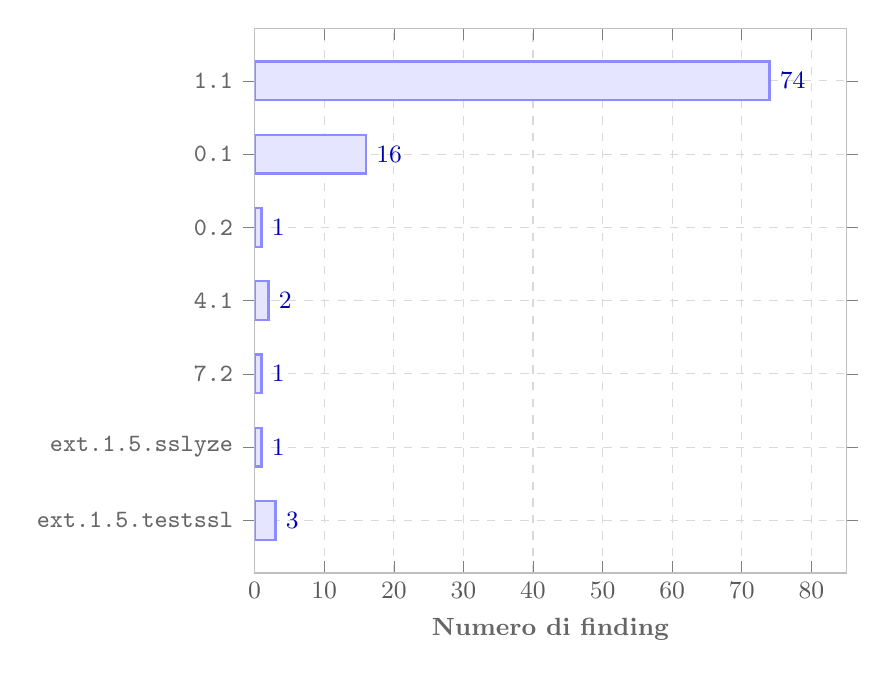
\begin{tikzpicture}
    \begin{axis}[
        xbar,
        width=0.75\textwidth, % <-- CORREZIONE: Lascia il 25% di spazio per le etichette laterali
        height=8.5cm,
        bar width=14pt,
        %
        % Setup Asse X
        xmin=0, xmax=85,
        xtick={0,10,20,30,40,50,60,70,80},
        xlabel={Numero di finding},
        xlabel style={font=\small\bfseries, text=gray!80!black},
        tick label style={font=\small, text=gray!70!black},
        %
        % Setup Asse Y
        symbolic y coords={{ext.1.5.testssl},{ext.1.5.sslyze},{7.2},{4.1},{0.2},{0.1},{1.1}},
        ytick=data,
        yticklabel style={font=\small\ttfamily, text=gray!80!black},
        enlarge y limits=0.12,
        %
        % Griglia
        grid=major,
        grid style={dashed, gray!30},
        axis line style={gray!50},
        %
        % Numeri a fianco delle barre
        nodes near coords,
        nodes near coords align={horizontal},
        every node near coord/.style={font=\small\bfseries, text=blue!70!black},
      ]

      \addplot[fill=blue!10, draw=blue!45, thick] coordinates {
          (3,{ext.1.5.testssl})
          (1,{ext.1.5.sslyze})
          (1,{7.2})
          (2,{4.1})
          (1,{0.2})
          (16,{0.1})
          (74,{1.1})
        };
    \end{axis}
  \end{tikzpicture}
  \caption{Distribuzione dei 98 finding per test nell'assessment di validazione.}
  \label{fig:finding-distribution}
  \par\smallskip
  {\small \noindent\textbf{Mini-guida: Figura~\ref{fig:finding-distribution}.}\\
    \texttt{Label:} \verb|\label{sec:coverage-idempotenza}| (\S5.3)\\
    \texttt{Ctrl+F:} cerca \texttt{98 finding} o \texttt{finding} in \S5.3\\
    \texttt{Azione:} inserire dopo la frase che introduce il conteggio totale dei finding, prima dell'analisi per dominio. }
\end{figure}

% ─── FIGURA L (8.9) -- Decision tree exit code CI/CD ─────────────────────────
\begin{figure}[ht]
  \centering
  \resizebox{\textwidth}{!}{%
    \begin{tikzpicture}[
        % Stili Gold Standard (niente dipendenze da classi esterne)
        base/.style={draw, rounded corners=1pt, inner sep=6pt, align=center, font=\small, minimum height=3.5ex},
        cmd/.style={base, fill=blue!5, draw=blue!40, font=\small\ttfamily, minimum width=18em},
        decision/.style={draw, shape=diamond, aspect=2.5, inner sep=2pt, align=center, font=\small, fill=orange!10, draw=orange!50},
        %
        % Stili per gli Exit Codes (Larghezza fissa per allineamento a colonna)
        code0/.style={base, fill=green!10, draw=green!50!black, minimum width=8.5em},
        code1/.style={base, fill=red!10, draw=red!60!black, minimum width=8.5em},
        code2/.style={base, fill=orange!10, draw=orange!60!black, minimum width=8.5em},
        code10/.style={base, fill=gray!15, draw=gray!60!black, minimum width=8.5em},
        %
        % Stili per le Actions (Larghezza fissa e generosa)
        act0/.style={base, fill=green!5, draw=green!40, minimum width=16em},
        act1/.style={base, fill=red!5, draw=red!40, minimum width=16em},
        act2/.style={base, fill=orange!5, draw=orange!40, minimum width=16em},
        act10/.style={base, fill=gray!5, draw=gray!40, minimum width=16em},
      ]

      %% ── Asse Centrale (Runner -> Comando -> Decisione) ────────────────────
      \node[base, fill=gray!10, draw=gray!40, font=\small\bfseries] (start) {Runner CI/CD};
      \node[cmd, below=3ex of start] (cmd) {apiguard run -{}-config config.yaml};
      \node[decision, below=3ex of cmd] (dec) {exit code?};

      %% ── Colonna Exit Codes (Ancorati in alto a sx, coordinate forzate) ────
      % Il primo è spostato a destra di 4em rispetto al centro del rombo
      \path (dec.south) ++(4em, -4ex) node[code0, anchor=north west] (e0) {\textbf{\texttt{0}: CLEAN}\\{\scriptsize tutti PASS/SKIP}};
      \path (e0.south west) ++(0, -2.5ex) node[code1, anchor=north west] (e1) {\textbf{\texttt{1}: FAIL}\\{\scriptsize almeno un FAIL}};
      \path (e1.south west) ++(0, -2.5ex) node[code2, anchor=north west] (e2) {\textbf{\texttt{2}: ERROR}\\{\scriptsize ERROR senza FAIL}};
      \path (e2.south west) ++(0, -2.5ex) node[code10, anchor=north west] (e10) {\textbf{\texttt{10}: INFRA}\\{\scriptsize errore infrastrutturale}};

      %% ── Colonna Actions (Ancorate esattamente a 3em a destra dei codici) ──
      \path (e0.east) ++(3em, 0) node[act0, anchor=west] (a0) {\textbf{Pipeline prosegue}\\{\scriptsize (merge / deploy consentito)}};
      \path (e1.east) ++(3em, 0) node[act1, anchor=west] (a1) {\textbf{Blocco merge/deploy}\\{\scriptsize Report allegato come artefatto}};
      \path (e2.east) ++(3em, 0) node[act2, anchor=west] (a2) {\textbf{Alert malfunzionamento}\\{\scriptsize Revisione manuale richiesta}};
      \path (e10.east) ++(3em, 0) node[act10, anchor=west] (a10) {\textbf{Diagnosi deployment}\\{\scriptsize Verifica \texttt{config.yaml}}};

      %% ── Frecce di Flusso Principale ───────────────────────────────────────
      % Uso -latex per garantire la punta della freccia pulita senza dipendere da ag-arr
      \draw[-latex, semithick] (start) -- (cmd);
      \draw[-latex, semithick] (cmd) -- (dec);

      %% ── Routing a Bus per le condizioni (Il tronco verticale) ─────────────
      \coordinate (bus-end) at (dec.south |- e10.west);
      \draw[gray!70, semithick] (dec.south) -- (bus-end);

      % Diramazioni orizzontali verso gli Exit Code (colorate)
      \draw[-latex, semithick, green!50!black] (dec.south |- e0.west) -- (e0.west);
      \fill[gray!70] (dec.south |- e0.west) circle (1.5pt);

      \draw[-latex, semithick, red!60!black] (dec.south |- e1.west) -- (e1.west);
      \fill[gray!70] (dec.south |- e1.west) circle (1.5pt);

      \draw[-latex, semithick, orange!60!black] (dec.south |- e2.west) -- (e2.west);
      \fill[gray!70] (dec.south |- e2.west) circle (1.5pt);

      \draw[-latex, semithick, gray!60!black] (dec.south |- e10.west) -- (e10.west);
      \fill[gray!70] (dec.south |- e10.west) circle (1.5pt);

      %% ── Frecce dalle Condizioni alle Azioni (colorate in scala) ───────────
      \draw[-latex, semithick, green!50!black] (e0.east) -- (a0.west);
      \draw[-latex, semithick, red!60!black] (e1.east) -- (a1.west);
      \draw[-latex, semithick, orange!60!black] (e2.east) -- (a2.west);
      \draw[-latex, semithick, gray!60!black] (e10.east) -- (a10.west);

    \end{tikzpicture}
  }%
  \caption{Routing degli exit code semantici (D6.P1) nella pipeline \gls{CI/CD}: 0 clean, 1 fail, 2 error, 10 infra.}
  \label{fig:cicd-decision-tree}
  \par\smallskip
  {\small \noindent\textbf{Mini-guida: Figura~\ref{fig:cicd-decision-tree}.}\\
    \texttt{Label:} \verb|\label{sec:devsecops}| (\S6.2)\\
    \texttt{Ctrl+F:} cerca \texttt{exit code} o \texttt{exit\_code} in \S6.2\\
    \texttt{Azione:} inserire nella sottosezione sugli exit code semantici, dopo il paragrafo che ne spiega la semantica. }
\end{figure}

% ─── FIGURA M (8.10) -- Piattaforma modulare ─────────────────────────────────
\begin{figure}[ht]
  \centering
  \resizebox{\textwidth}{!}{%
    \begin{tikzpicture}[
        % Distanza puramente tipografica (Gold Standard): 5ex verticale, 3.5em orizzontale
        node distance=5ex and 3.5em,
        %
        % Stili di base
        base/.style={draw, rounded corners=2pt, inner sep=6pt, align=center, font=\small, minimum height=3.5ex},
        %
        % Core (Blu)
        core/.style={base, fill=blue!8, draw=blue!45, minimum width=17em, thick},
        %
        % Moduli Satelliti
        active/.style={base, fill=green!10, draw=green!50!black, minimum width=8.5em},
        planned/.style={base, fill=gray!4, draw=gray!40, dashed, minimum width=8.5em, font=\small\itshape},
        %
        % Stili Frecce
        arr-active/.style={-latex, thick, green!50!black},
        arr-planned/.style={-latex, thick, dashed, gray!50}
      ]

      %% ── Core immutabile (Centro) ──────────────────────────────────────────
      \node[core] (core) {
      \textbf{Core: infrastruttura immutabile}\\
      {\scriptsize Engine \textbar{} DAG Scheduler \textbar{} EvidenceStore}\\
      {\scriptsize TargetContext \textbar{} BaseTest \textbar{} BaseConnector}
      };

      %% ── Moduli Satelliti (A stella) ───────────────────────────────────────
      % Modulo attivo (Sopra)
      \node[active, above=of core] (rest) {\textbf{REST / OAS}\\{\scriptsize (attivo)}};

      % Moduli pianificati (Destra, Sotto, Sinistra)
      \node[planned, right=of core] (gql) {\textbf{GraphQL}\\{\scriptsize (pianificato)}};
      \node[planned, below=of core] (grpc) {\textbf{gRPC}\\{\scriptsize (pianificato)}};
      \node[planned, left=of core] (ws) {\textbf{WebSocket}\\{\scriptsize (pianificato)}};

      %% ── Frecce di Collegamento (Convergenti verso il Core) ────────────────
      \draw[arr-active] (rest.south) -- (core.north);
      \draw[arr-planned] (gql.west) -- (core.east);
      \draw[arr-planned] (grpc.north) -- (core.south);
      \draw[arr-planned] (ws.east) -- (core.west);

      %% ── Legenda e Note ────────────────────────────────────────────────────
      % Distanza puramente tipografica anche qui (4ex)
      \node[font=\small, text=gray!80!black, below=4ex of grpc, align=center] (note) {
      frecce continue: modulo attivo \quad frecce tratteggiate: moduli pianificati\\[1ex]
      {\itshape Il discovery dinamico via \texttt{pkgutil} permette il caricamento trasparente di moduli di terze parti}
      };

    \end{tikzpicture}
  }%
  \caption{Evoluzione di APIGuard Assurance verso una piattaforma modulare: core immutabile e moduli di protocollo intercambiabili.}
  \label{fig:modular-platform}
  \par\smallskip
  {\small \noindent\textbf{Mini-guida: Figura~\ref{fig:modular-platform}.}\\
    \texttt{Label:} \verb|\label{sec:sviluppi-futuri}| (\S6.3)\\
    \texttt{Ctrl+F:} cerca \texttt{plugin} o \texttt{pkgutil} in \S6.3\\
    \texttt{Azione:} inserire nella sottosezione sul plugin system, come chiusura visiva delle future work. }
\end{figure}


% ─── FIGURA N1 -- Mappa di Copertura ─────────────────────────────────────────
%
% Mostra: quali test sono attivi per dominio, strategia Box Gradient,
%         esito (PASS/FAIL/SKIP) nell'assessment di validazione v0.1.0.
% Valore aggiunto: nessuna tabella esistente combina test individuali + strategia
%                  + esito in un'unica vista.
%
\begin{figure}[ht]
  \centering
  \resizebox{\textwidth}{!}{%
    \begin{tikzpicture}[
        % Spaziatura compatta
        node distance=1.5ex and 0.4em,
        %
        % Stili di base: inner sep portato a 4pt per allontanare il testo dai bordi
        base/.style={draw, rounded corners=1.5pt, align=center, inner sep=4pt},
        %
        % Etichetta di dominio: Altezza aumentata a 5.2ex
        dom/.style={base, fill=gray!10, draw=gray!50, minimum width=11.5em, minimum height=5.2ex, font=\footnotesize\bfseries},
        %
        % Stili Esiti
        pass/.style={fill=green!10, draw=green!50!black},
        fail/.style={fill=red!10, draw=red!60!black},
        skip/.style={fill=gray!15, draw=gray!50},
        %
        % Nodi test nativi: Altezza aumentata per mantenere l'allineamento a griglia
        tst/.style={base, minimum width=3.5em, minimum height=5.2ex, font=\footnotesize\ttfamily},
        %
        % Nodi test esterni: Altezza aumentata a 5.2ex
        ext/.style={base, minimum width=5em, minimum height=5.2ex, font=\footnotesize\ttfamily\itshape},
        %
        % Placeholder per D5
        inact/.style={base, draw=gray!35, dashed, fill=gray!4, minimum width=8em, minimum height=5.2ex, font=\footnotesize\itshape, text=gray!70!black},
      ]

      %% ── D0: Discovery ─────────────────────────────────────────────────────
      \node[dom] (d0) {D0: Discovery\\[-1pt]{\scriptsize B\,|\,G\quad P0--P1}};

      \node[tst, fail, right=1.5em of d0] (t01)  {\texttt{0.1}};
      \node[tst, fail, right=of t01]      (t02)  {\texttt{0.2}};
      \node[tst, skip, right=of t02]      (t03)  {\texttt{0.3}};
      \node[ext, pass, right=of t03]      (te01) {\texttt{ext.0.1}\\[-2pt]{\scriptsize nuclei}};

      %% ── D1: Authentication ────────────────────────────────────────────────
      \node[dom, below=1.5ex of d0.south west, anchor=north west] (d1)
      {D1: Authentication\\[-1pt]{\scriptsize B\,|\,G\quad P0--P1}};

      \node[tst, fail, right=1.5em of d1] (t11)   {\texttt{1.1}};
      \node[tst, pass, right=of t11]      (t14)   {\texttt{1.4}};
      \node[tst, pass, right=of t14]      (t15)   {\texttt{1.5}};
      \node[tst, skip, right=of t15]      (t16)   {\texttt{1.6}};
      \node[ext, fail, right=of t16]      (te15s) {\texttt{ext.1.5}\\[-2pt]{\scriptsize sslyze}};
      \node[ext, fail, right=of te15s]    (te15t) {\texttt{ext.1.5}\\[-2pt]{\scriptsize testssl}};

      %% ── D2: Authorization ─────────────────────────────────────────────────
      \node[dom, below=1.5ex of d1.south west, anchor=north west] (d2)
      {D2: Authorization\\[-1pt]{\scriptsize G\quad P1--P2}};

      \node[tst, pass, right=1.5em of d2] (t21) {\texttt{2.1}};

      %% ── D3: Data Integrity ────────────────────────────────────────────────
      \node[dom, below=1.5ex of d2.south west, anchor=north west] (d3)
      {D3: Data Integrity\\[-1pt]{\scriptsize G\quad P2}};

      \node[tst, pass, right=1.5em of d3] (t33) {\texttt{3.3}};

      %% ── D4: Availability ──────────────────────────────────────────────────
      \node[dom, below=1.5ex of d3.south west, anchor=north west] (d4)
      {D4: Availability\\[-1pt]{\scriptsize G\,|\,W\quad P1--P2}};

      \node[tst, fail, right=1.5em of d4] (t41) {\texttt{4.1}};
      \node[tst, pass, right=of t41]      (t42) {\texttt{4.2}};
      \node[tst, pass, right=of t42]      (t43) {\texttt{4.3}};

      %% ── D5: Observability — nessun test attivo (Milestone 2) ──────────────
      \node[dom, fill=gray!4, draw=gray!35, below=1.5ex of d4.south west, anchor=north west] (d5)
      {D5: Observability\\[-1pt]{\scriptsize W\quad P3\quad\textit{(M2)}}};

      \node[inact, right=1.5em of d5] (td5) {nessun test attivo};

      %% ── D6: Hardening ─────────────────────────────────────────────────────
      \node[dom, below=1.5ex of d5.south west, anchor=north west] (d6)
      {D6: Hardening\\[-1pt]{\scriptsize W\quad P2--P3}};

      \node[tst, pass, right=1.5em of d6] (t62) {\texttt{6.2}};
      \node[tst, pass, right=of t62]      (t64) {\texttt{6.4}};

      %% ── D7: Business Logic ────────────────────────────────────────────────
      \node[dom, below=1.5ex of d6.south west, anchor=north west] (d7)
      {D7: Business Logic\\[-1pt]{\scriptsize G\quad P2}};

      \node[tst, fail, right=1.5em of d7] (t72) {\texttt{7.2}};

      %% ── Legenda ──────────────────────────────────────────────────────────
      \node[tst, pass, below=3.5ex of d7.south west, anchor=north west] (lg-pass) {\texttt{PASS}};
      \node[tst, fail, right=0.8em of lg-pass] (lg-fail) {\texttt{FAIL}};
      \node[tst, skip, right=0.8em of lg-fail] (lg-skip) {\texttt{SKIP}};
      \node[ext, pass, right=0.8em of lg-skip] (lg-ext)  {\textit{Esterno}};
      \node[font=\footnotesize\itshape, text=gray!70!black, right=0.8em of lg-ext] {corsivo = test esterno tramite connector};

    \end{tikzpicture}
  }%
  \caption{Mappa di copertura dell'assessment di validazione (v0.1.0): test attivi per dominio di assurance, strategia Box Gradient (D3.P3) ed esito (\texttt{PASS}/\texttt{FAIL}/\texttt{SKIP}). I test esterni, eseguiti tramite connector, sono riportati in corsivo.}
  \label{fig:coverage-map}
  \par\smallskip
  {\small \noindent\textbf{Mini-guida: Figura~\ref{fig:coverage-map}.}\\
    \texttt{Label:} \verb|\label{sec:coverage-idempotenza}| (\S5.3)\\
    \texttt{Ctrl+F:} \texttt{L'assessment ha prodotto 98 finding distribuiti}\\
    \texttt{Azione:} inserire all'inizio di \S5.3.1 (Analisi dei Risultati per Dominio), prima della lettura verbale degli esiti.}
\end{figure}


% ─── FIGURA N2 -- Tre Canali Tipizzati del TestContext ───────────────────────
%
% Mostra: la struttura interna del TestContext (canale token, teardown, shared)
%         con API, ruoli costanti e convenzione di naming.
% Valore aggiunto: fig:architettura-apiguard mostra il TestContext come nodo
%                  atomico; questa figura ne mostra la struttura interna a tre canali
%                  e il pattern di accesso, non rappresentato altrove.
%
\begin{figure}[ht]
  \centering
  \resizebox{\textwidth}{!}{%
    \begin{tikzpicture}[
        % Distanze compatte per fermare il downscaling di resizebox
        node distance=1.2ex and 1em,
        %
        % Intestazione del canale
        ch-hdr/.style={draw=green!60!black, fill=green!18, rounded corners=1.5pt,
            minimum width=11.5em, font=\small\bfseries, align=center},
        %
        % Riga di metodo/dato dentro il canale
        ch-row/.style={draw=green!50!black, fill=green!7, rounded corners=1.5pt,
            minimum width=11.5em, minimum height=18pt,
            inner sep=4pt, font=\footnotesize\ttfamily, align=left},
        %
        % Blocco API
        ch-api/.style={draw=gray!40, fill=gray!10, rounded corners=1.5pt,
            minimum width=11.5em, inner sep=4pt, font=\footnotesize, align=left},
        %
        % Badge di fase (quando il canale viene usato)
        ph-badge/.style={draw=gray!50, fill=gray!15, rounded corners=1.5pt,
            minimum width=11.5em, inner sep=3pt, font=\footnotesize\bfseries, align=center},
      ]

      %% ─────────────────────────────────────────────────────────────────────
      %% Canale Token (sinistra)
      %% ─────────────────────────────────────────────────────────────────────
      \node[ch-hdr] (tok-hdr) {Canale Token};

      \node[ch-row, below=0.6ex of tok-hdr] (tok-r1) {\texttt{ROLE\_ADMIN}};
      \node[ch-row, below=0.6ex of tok-r1]  (tok-r2) {\texttt{ROLE\_USER\_A}};
      \node[ch-row, below=0.6ex of tok-r2]  (tok-r3) {\texttt{ROLE\_USER\_B}};

      \node[ch-api, below=0.6ex of tok-r3] (tok-api) {
        \texttt{set\_token(role, tok)}\\[1pt]
        \texttt{get\_token(role) \textrightarrow{} tok}\\[1pt]
        \texttt{has\_token(role) \textrightarrow{} bool}
      };

      \node[ph-badge, below=1.2ex of tok-api] (tok-ph) {Fase~5: test autenticati\\scrivono e leggono};

      %% ─────────────────────────────────────────────────────────────────────
      %% Canale Teardown LIFO (centro)
      %% ─────────────────────────────────────────────────────────────────────
      \node[ch-hdr, right=of tok-hdr] (td-hdr) {Canale Teardown \footnotesize[LIFO]};

      \node[ch-row, below=0.6ex of td-hdr] (td-r1) {push(fn\_C)};
      \node[ch-row, below=0.6ex of td-r1]  (td-r2) {push(fn\_B)};
      \node[ch-row, below=0.6ex of td-r2]  (td-r3) {push(fn\_A)};

      \node[ch-api, below=0.6ex of td-r3] (td-api) {
      \texttt{push\_teardown(callable)}\\[1pt]
      {\itshape drain order:}\\[1pt]
      \texttt{fn\_A \textrightarrow{} fn\_B \textrightarrow{} fn\_C}
      };

      \node[ph-badge, below=1.2ex of td-api] (td-ph) {Fase~5: push\\Fase~6: drain inv.};

      %% ─────────────────────────────────────────────────────────────────────
      %% Canale Shared Data (destra)
      %% ─────────────────────────────────────────────────────────────────────
      \node[ch-hdr, right=of td-hdr] (sh-hdr) {Canale Shared Data};

      \node[ch-row, below=0.6ex of sh-hdr] (sh-r1) {\texttt{"1.1.token"}};
      \node[ch-row, below=0.6ex of sh-r1]  (sh-r2) {\texttt{"1.1.repos"}};
      \node[ch-row, below=0.6ex of sh-r2]  (sh-r3) {\texttt{"ext.0.1.hits"}};

      \node[ch-api, below=0.6ex of sh-r3] (sh-api) {
        \texttt{set\_shared("{id}.{k}", v)}\\[1pt]
        \texttt{get\_shared("{id}.{k}")}\\[1pt]
        \texttt{~~\textrightarrow{} v}
      };

      \node[ph-badge, below=1.2ex of sh-api] (sh-ph) {Fase~5: produttore scrive\\batch successivi leggono};

      %% ── Sfondo per i tre canali ──────────────────────────────────────────
      \begin{scope}[on background layer]
        \node[draw=green!50!black, fill=green!3, rounded corners=3pt, inner sep=6pt,
          fit=(tok-hdr)(tok-r1)(tok-r2)(tok-r3)(tok-api)(tok-ph)] {};
        \node[draw=green!50!black, fill=green!3, rounded corners=3pt, inner sep=6pt,
          fit=(td-hdr)(td-r1)(td-r2)(td-r3)(td-api)(td-ph)] {};
        \node[draw=green!50!black, fill=green!3, rounded corners=3pt, inner sep=6pt,
          fit=(sh-hdr)(sh-r1)(sh-r2)(sh-r3)(sh-api)(sh-ph)] {};
      \end{scope}

      %% ── Intestazione globale (TestContext) ───────────────────────────────
      % Larghezza dinamica usando il fit tra il primo e l'ultimo header per centratura perfetta
      \node[draw=green!60!black, fill=green!25, rounded corners=2pt,
        minimum width=36.5em, font=\small\bfseries, align=center,
        above=3ex of td-hdr.north] (tc-master)
      {\texttt{TestContext} [mutable]: tre canali tipizzati con responsabilità distinte};

    \end{tikzpicture}
  }%
  \caption{Struttura interna del \texttt{TestContext} (D1.P3): i tre canali tipizzati con le rispettive \gls{API} di accesso, le chiavi costanti per il canale token, il pattern di naming per il canale shared e l'ordinamento \gls{LIFO} del canale teardown.}
  \label{fig:testcontext-channels}
  \par\smallskip
  {\small \noindent\textbf{Mini-guida: Figura~\ref{fig:testcontext-channels}.}\\
    \texttt{Label:} \verb|\label{subsec:split-state-impl}| (\S4.4)\\
    \texttt{Ctrl+F:} \texttt{TestContext è mutabile, ma l'accesso non avviene}\\
    \texttt{Azione:} inserire dopo il paragrafo che descrive i tre canali, prima della sezione sul DAGScheduler. }
\end{figure}


% ─── FIGURA N4 -- Gerarchia delle Eccezioni ──────────────────────────────────
%
% Mostra: l'albero delle 11 classi custom con colore per categoria
%         (bloccanti / recuperate / CLI) e file di definizione.
% Valore aggiunto: la Tabella tab:exception-hierarchy elenca le classi in modo
%                  piatto; la struttura ad albero con la radice comune e la
%                  distinzione cromatica tra bloccanti e recuperate non è
%                  rappresentata altrove.
%
\begin{figure}[ht]
  \centering
  \resizebox{\textwidth}{!}{%
    \begin{tikzpicture}[
        % Distanze ridotte: ora usiamo la larghezza per risparmiare altezza
        node distance=0.8ex and 1.5em,
        %
        % Stili di base: 19em di larghezza ci permette di tenere tutto su 1 riga
        base/.style={draw, rounded corners=1.5pt, inner sep=5pt, text width=19em, align=left, font=\small},
        %
        root/.style={draw=gray!50, fill=gray!10, rounded corners=2pt, inner sep=6pt, align=center, minimum width=9em},
        %
        blk/.style={base, fill=red!6, draw=red!50},
        rec/.style={base, fill=orange!8, draw=orange!50},
        cli/.style={base, fill=gray!8, draw=gray!50},
        %
        % Categorie snellite
        cat-lbl/.style={align=right, text width=8em},
        %
        % Fili sottili ed eleganti
        tree/.style={-latex, gray!60, semithick, rounded corners=2pt},
        fork/.style={gray!60, semithick, rounded corners=2pt}
      ]

      %% ── 1. Nodi Eccezioni a singola riga (Colonna di Destra) ──────────────

      % Bloccanti
      \node[blk] (b1) {\texttt{ConfigurationError} \hfill {\footnotesize\color{red!70!black}[Fase 1]}};
      \node[blk, below=0.8ex of b1] (b2) {\texttt{OpenAPILoadError} \hfill {\footnotesize\color{red!70!black}[Fase 2]}};
      \node[blk, below=0.8ex of b2] (b3) {\texttt{DAGCycleError} \hfill {\footnotesize\color{red!70!black}[Fase 4]}};
      \node[blk, below=0.8ex of b3] (b4) {\texttt{AuthenticationSetupError} \hfill {\footnotesize\color{red!70!black}[auth helper]}};

      % Recuperate (Staccate leggermente dal gruppo sopra)
      \node[rec, below=2.5ex of b4] (r1) {\texttt{SecurityClientError} \hfill {\footnotesize\color{orange!70!black}[Fase 5 \textrightarrow{} ERROR]}};
      \node[rec, below=0.8ex of r1] (r2) {\texttt{ExternalToolError} \hfill {\footnotesize\color{orange!70!black}[Fase 5 \textrightarrow{} ERROR]}};
      \node[rec, below=0.8ex of r2] (r3) {\texttt{TeardownError} \hfill {\footnotesize\color{orange!70!black}[Fase 6 \textrightarrow{} WARN]}};
      \node[rec, below=0.8ex of r3] (r4) {\texttt{GatewayAdapterError} \hfill {\footnotesize\color{orange!70!black}[gateway/base.py]}};

      % CLI (Staccate leggermente)
      \node[cli, below=2.5ex of r4] (c1) {\texttt{SeedGeneratorFetchError} \hfill {\footnotesize\color{gray!70!black}[exit code 10]}};
      \node[cli, below=0.8ex of c1] (c2) {\texttt{SeedGeneratorParseError} \hfill {\footnotesize\color{gray!70!black}[exit code 10]}};

      %% ── 2. Etichette Categorie (Colonna Centrale) ─────────────────────────
      % Ancorate matematicamente a metà altezza dei rispettivi gruppi

      \path (b1.north west) -- (b4.south west) node[midway, left=1.5em, anchor=east, cat-lbl, text=red!70!black] (lbl-blk) {
      \textbf{Bloccanti}\\ {\footnotesize (Fasi 1--4)}\\[1pt] {\footnotesize\normalfont\color{gray!70!black} bloccano l'avvio}
      };

      \path (r1.north west) -- (r4.south west) node[midway, left=1.5em, anchor=east, cat-lbl, text=orange!70!black] (lbl-rec) {
      \textbf{Recuperate}\\ {\footnotesize (Fasi 5--6)}\\[1pt] {\footnotesize\normalfont\color{gray!70!black} ERROR / WARNING}
      };

      \path (c1.north west) -- (c2.south west) node[midway, left=1.5em, anchor=east, cat-lbl, text=gray!60!black] (lbl-cli) {
      \textbf{CLI}\\ {\footnotesize \texttt{generate-seed}}\\[1pt] {\footnotesize\normalfont\color{gray!70!black} standalone}
      };

      %% ── 3. Radice (Colonna Sinistra) ──────────────────────────────────────
      \path (lbl-blk.north west) -- (lbl-cli.south west) node[midway, left=1.5em, anchor=east, root] (root) {
      \textbf{\texttt{ToolBaseError}}\\[2pt]{\footnotesize\itshape(classe astratta)}
      };

      %% ── 4. Geometrie dei Cavi (Routing) ───────────────────────────────────

      % Dal padre alle 3 categorie
      \draw[tree] (root.east) -- ++(0.75em, 0) |- (lbl-blk.west);
      \draw[tree] (root.east) -- ++(0.75em, 0) |- (lbl-rec.west);
      \draw[tree] (root.east) -- ++(0.75em, 0) |- (lbl-cli.west);

      % Dal nodo "Bloccanti" ai 4 figli
      \coordinate (Fblk) at ([xshift=0.75em]lbl-blk.east);
      \draw[fork] (lbl-blk.east) -- (Fblk);
      \draw[tree] (Fblk) |- (b1.west);
      \draw[tree] (Fblk) |- (b2.west);
      \draw[tree] (Fblk) |- (b3.west);
      \draw[tree] (Fblk) |- (b4.west);

      % Dal nodo "Recuperate" ai 4 figli
      \coordinate (Frec) at ([xshift=0.75em]lbl-rec.east);
      \draw[fork] (lbl-rec.east) -- (Frec);
      \draw[tree] (Frec) |- (r1.west);
      \draw[tree] (Frec) |- (r2.west);
      \draw[tree] (Frec) |- (r3.west);
      \draw[tree] (Frec) |- (r4.west);

      % Dal nodo "CLI" ai 2 figli
      \coordinate (Fcli) at ([xshift=0.75em]lbl-cli.east);
      \draw[fork] (lbl-cli.east) -- (Fcli);
      \draw[tree] (Fcli) |- (c1.west);
      \draw[tree] (Fcli) |- (c2.west);

    \end{tikzpicture}
  }%
  \caption{Gerarchia delle 11 eccezioni custom di APIGuard Assurance (D4.P4): eccezioni bloccanti che interrompono lo startup (Fasi~1--4, rosso), eccezioni recuperate localmente che producono \texttt{TestResult(ERROR/WARNING)} (Fasi~5--6, oro), e classi specifiche del comando \gls{CLI} \texttt{generate-seed} (grigio). Tutte ereditano da \texttt{ToolBaseError}.}
  \label{fig:exception-hierarchy}
  \par\smallskip
  {\small \noindent\textbf{Mini-guida: Figura~\ref{fig:exception-hierarchy}.}\\
    \texttt{Label:} \verb|\label{subsec:exception-hierarchy}| (\S4.1.2)\\
    \texttt{Ctrl+F:} \texttt{Tutte le eccezioni del tool ereditano da ToolBaseError}\\
    \texttt{Azione:} inserire prima o dopo la Tabella~\ref{tab:exception-hierarchy}, come complemento visivo alla struttura piatta della tabella. }
\end{figure}


% ─── FIGURA (Pipeline Flow) ──────────────────────────────────────────────────
\begin{figure}[ht]
  \centering
  % NIENTE \resizebox: ottimizzato orizzontalmente per far rientrare la grafica 
  % nei margini e lasciare che i font \footnotesize si renderizzino alla loro grandezza reale.
  \begin{tikzpicture}[
      % Distanza orizzontale compatta per accorciare le frecce laterali
      node distance=3.5ex and 4.5em,
      %
      % Stili di base
      base/.style={draw, rounded corners=1.5pt, inner sep=5pt, align=center, font=\small, minimum height=4.5ex},
      %
      % Stili Fasi (Colonna Sinistra)
      phase-startup/.style={base, fill=blue!7, draw=blue!40, minimum width=13.5em},
      phase-exec/.style={base, fill=green!7, draw=green!45, minimum width=13.5em},
      %
      % Stili Errori (Colonna Destra)
      err-stop/.style={base, fill=red!6, draw=red!50, minimum width=12.5em},
      err-warn/.style={base, fill=orange!8, draw=orange!50, minimum width=12.5em},
      %
      % Terminali (Inizio/Fine)
      term/.style={draw=gray!50, fill=gray!15, ellipse, minimum height=3.5ex, inner sep=5pt, align=center, font=\footnotesize\ttfamily},
      %
      % Testi secondari sulle frecce (inner sep=3pt aggiunto per distaccarle dai fili)
      lbl/.style={font=\footnotesize\itshape, text=gray!70!black, inner sep=3pt},
      %
      % Frecce ortogonali
      arr-ok/.style={-latex, semithick, gray!70!black},
      arr-ko/.style={-latex, semithick, red!60!black},
      arr-warn/.style={-latex, semithick, dashed, orange!80!black},
      %
      % Sfondi per raggruppamento dinamico (Libreria fit)
      bg-startup/.style={draw=blue!30, fill=blue!3, dashed, rounded corners=3pt, inner sep=10pt},
      bg-exec/.style={draw=green!35, fill=green!2, dashed, rounded corners=3pt, inner sep=10pt}
    ]

    %% ── Terminale di avvio ─────────────────────────────────────────────────
    \node[term] (start) {apiguard run};

    %% ── Fasi 1-4 (zona startup, bloccanti) ─────────────────────────────────
    % Spazio a 8ex per creare il corridoio d'ingresso
    \node[phase-startup, below=8ex of start] (p1) {\textbf{Fase~1:} Inizializzazione\\{\footnotesize\texttt{config/loader.py}}};
    \node[phase-startup, below=of p1]    (p2) {\textbf{Fase~2:} OpenAPI Discovery\\{\footnotesize\texttt{discovery/openapi.py}}};
    \node[phase-startup, below=of p2]    (p3) {\textbf{Fase~3:} Costruzione Contesti\\{\footnotesize\texttt{engine.py}}};
    \node[phase-startup, below=of p3]    (p4) {\textbf{Fase~4:} Test Discovery e \gls{DAG}\\{\footnotesize\texttt{registry.py, dag.py}}};

    %% ── Fasi 5-7 (zona esecuzione, non bloccanti) ──────────────────────────
    % GAP ridotto: spazio a 9ex (lascia 5ex netti tra i due box di background)
    \node[phase-exec, below=9ex of p4] (p5) {\textbf{Fase~5:} Esecuzione (per test)\\{\footnotesize\texttt{engine.py}}};
    \node[phase-exec, below=of p5]   (p6) {\textbf{Fase~6:} Teardown \gls{LIFO}\\{\footnotesize\texttt{core/context.py}}};
    \node[phase-exec, below=of p6]   (p7) {\textbf{Fase~7:} Report\\{\footnotesize\texttt{report/renderer.py}}};

    %% ── Terminale di uscita ────────────────────────────────────────────────
    \node[term, below=5ex of p7] (end) {exit code: 0 / 1 / 2 / 10};

    %% ── Rami KO → STOP (fasi bloccanti) posizionati prima degli sfondi ─────
    \node[err-stop, right=4.5em of p1] (s1) {\texttt{ConfigurationError}\\{\footnotesize avvio interrotto}};
    \node[err-stop, right=4.5em of p2] (s2) {\texttt{OpenAPILoadError}\\{\footnotesize avvio interrotto}};
    \node[err-stop, right=4.5em of p4] (s4) {\texttt{DAGCycleError}\\{\footnotesize avvio interrotto}};

    %% ── Rami errore recuperabile (fasi 5, 6) ───────────────────────────────
    \node[err-warn, right=4.5em of p5] (w5) {\texttt{TestResult(ERROR)}\\{\footnotesize isolato, pipeline prosegue}};
    \node[err-warn, right=4.5em of p6] (w6) {\texttt{TeardownError}\\{\footnotesize \texttt{WARNING} strutturato}};

    %% ── Sfondi per le due zone ─────────────────────────────────────────────
    \begin{scope}[on background layer]
      \node[bg-startup, fit=(p1)(p2)(p3)(p4)] (grp-startup) {};
      \node[bg-exec, fit=(p5)(p6)(p7)] (grp-exec) {};
    \end{scope}

    %% ── ETICHETTE DI GRUPPO (Avvicinate all'asse e centrate in Y) ──────────
    % xshift=-0.6em le avvicina notevolmente alla freccia centrale
    % yshift=3ex solleva la prima etichetta al centro matematico del gap superiore.
    \node[font=\footnotesize\bfseries, text=blue!70!black, anchor=east]
    at ([xshift=-0.6em, yshift=3ex]grp-startup.north) {Fasi 1-4 (bloccanti)};

    % yshift=2.5ex solleva la seconda etichetta al centro matematico del gap centrale di 5ex netti.
    \node[font=\footnotesize\bfseries, text=green!70!black, anchor=east]
    at ([xshift=-0.6em, yshift=2.5ex]grp-exec.north) {Fasi 5-7 (non bloccanti)};

    %% ── Frecce asse principale ─────────────────────────────────────────────
    \draw[arr-ok] (start) -- (p1);
    \draw[arr-ok] (p1) -- node[midway, right, lbl] {OK} (p2);
    \draw[arr-ok] (p2) -- node[midway, right, lbl] {OK} (p3);
    \draw[arr-ok] (p3) -- node[midway, right, lbl] {OK} (p4);
    \draw[arr-ok] (p4) -- node[midway, right, lbl] {OK} (p5);
    \draw[arr-ok] (p5) -- (p6);
    \draw[arr-ok] (p6) -- node[midway, right, lbl] {OK} (p7);
    \draw[arr-ok] (p7) -- (end);

    %% ── Frecce Laterali (Centrate nello spazio vuoto ricalibrato a pos=0.55) 
    % Il valore 0.55 arretra i testi rispetto al 0.65 precedente, staccandoli dai riquadri di destra
    \draw[arr-ko] (p1.east) -- node[pos=0.55, above, lbl, text=red!70!black] {KO} (s1.west);
    \draw[arr-ko] (p2.east) -- node[pos=0.55, above, lbl, text=red!70!black] {KO} (s2.west);
    \draw[arr-ko] (p4.east) -- node[pos=0.55, above, lbl, text=red!70!black] {KO} (s4.west);

    \draw[arr-warn] (p5.east) -- node[pos=0.55, above, align=center, lbl, text=orange!80!black] {eccezione\\interna} (w5.west);
    \draw[arr-warn] (p6.east) -- node[pos=0.55, above, align=center, lbl, text=orange!80!black] {cleanup\\parziale} (w6.west);

  \end{tikzpicture}
  \caption{Flusso della pipeline a sette fasi (D4.P3, D4.P4): la zona di startup (Fasi~1-4) è bloccante, un errore in una qualsiasi di esse interrompe l'avvio; la zona di esecuzione (Fasi~5-7) è non bloccante, ogni malfunzionamento è recuperato localmente senza invalidare i risultati già prodotti. Frecce continue: percorso nominale; frecce tratteggiate: errori recuperati con \texttt{WARNING}.}
  \label{fig:pipeline-flow}
\end{figure}